In what follows we decided to drop the first type of solution from the dataset
(i.e.\ \texttt{solutions} $= 0$) since it looks ``too perfect'' for the
analysis and might spoil the final results (also, removing a restricted number
of samples does not change the underlying distribution, as shown earlier).

\subsection{Test and Validation Sets}\label{sec:reg:test_val}

The splits for training and test sets have been chosen in order to keep samples
coming from the same \texttt{solutions} inside the same set in order to
maintain a good balance in the distribution of the variables.
In other words, we choose the samples in the test and training sets by first
subsampling the unique values of the \texttt{solutions} column, then we split
them into separate sets, and ultimately we assign the corresponding samples to
the splits.

\begin{figure}[htbp]
  \centering
  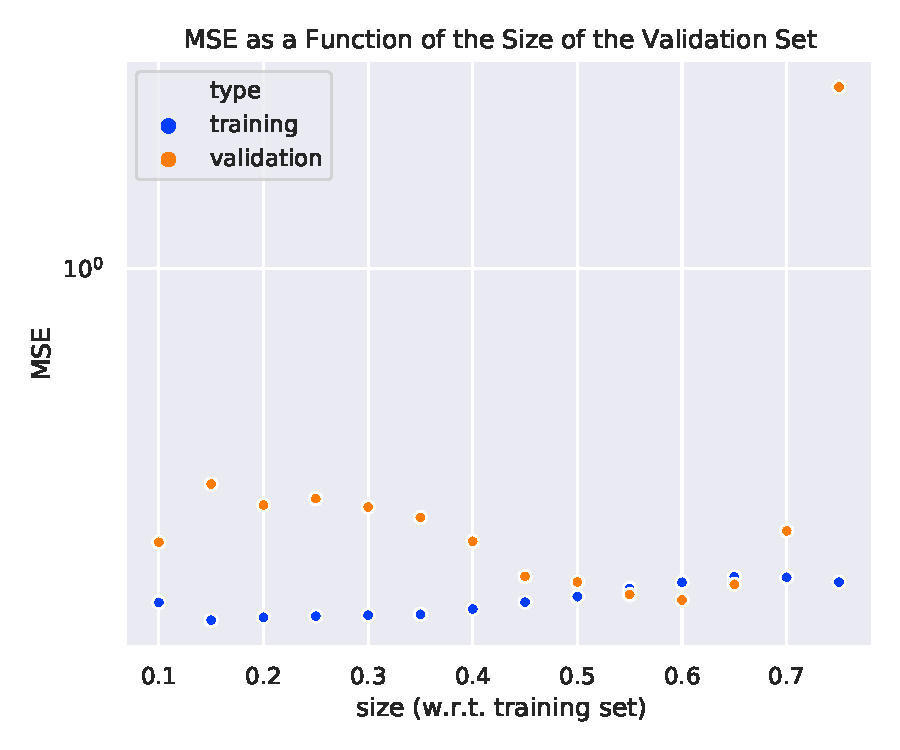
\includegraphics[width=0.4\textwidth]{img/training-validation-errors}
  \caption{MSE in training and validation for several sizes of the validation set.}
  \label{fig:reg:validation_size}
\end{figure}
We first decide to subsample around 10\% of the solutions for the test set and
keep the remaining 90\% for training and validation.
Notice that we do not use cross-validation in this case since the number of
samples is very restricted and we still want to keep samples coming from the
same \texttt{solutions} in the same split.

We chose the size of the validation set to be around 10\% of the total training
set as it is typical for datasets of this dimension where most of the samples
should be assigned to training.

Another motivation for the choice is to try to minimise the error (the Mean
Squared Error, MSE) made when fitting a linear regression on decreasing size of
the set effectively used for training, after removing the validation split:
this may clearly not work for anything different from a linear model, but it is
however a good starting point.
In \Cref{fig:reg:validation_size} we show training and validation MSE for
different sizes of the validation set (with respect to the total training set).
In order to keep a reasonable amount of samples in the training split and to
contain the validation MSE as much as possible, we finally take the already
announced 10\% of the unique \texttt{solutions} in the validation set.
\begin{table}[htbp]
\centering
\begin{tabular}{@{}ccc@{}}
\toprule
           & \multicolumn{2}{c}{\textbf{total dataset}} \\
\midrule
           & \textit{samples}    & \textit{fraction}    \\
\midrule
training   & 579                 & 81\%                 \\
validation & 61                  & 8\%                  \\
test       & 78                  & 11\%                 \\
\bottomrule
\end{tabular}
\caption{Summary of the train/validation/test splits.}
\label{tab:reg:splits}
\end{table}
In \Cref{tab:reg:splits} we give a schematic summary of the final choice for
training, validation and test sets.

\subsection{Preliminary Linear Regression Analysis}\label{sec:reg:prel}

Before moving to the ML analysis, we first perform a preliminary study using
linear regression to infer properties of the variables which may play a role in
the ML algorithms.
From now on we shall consider the training data as robustly scaled against the
outliers (i.e.\ we pre-process using \texttt{sklearn.RobustScaler}). 

We first fit the linear regression algorithm on the train set and then compute
the predictions on the three splits to study the values of the coefficients,
their associated standard error, t-statistics and probabilities of being
different from zero.
For this and the ML analysis we do not fit the intercept of the models since
the variables cannot vanish altogether: the intercept has therefore no
interpretation in discovering a structure in the values or performing
regression.

The study revealed that when considering the full dataset, all the variables
should be considered for regression as the coefficients are non vanishing (with
95\% confidence), mostly due to the very large variance of the data which
allows only very precise (i.e.\ very small standard errors) determinations of
the coefficients.
The same study performed on the usual separate ranges of \texttt{weight} showed
that when considering \texttt{weight} $\ge 1.5$ the variable \texttt{type} is
not necessary to the fit and we cannot reject the hypothesis of a vanishing
coefficient for such feature: this in fact reflect one of the properties
discovered during the EDA and summarised in \Cref{tab:eda:weight} where we
showed that for \texttt{weight} $\ge 1.5$ only one \texttt{type} is present in
the dataset and does not influence the final predictions.
We will however keep such feature inside the training variables since a further
study on the full dataset without the categorical variable showed that
predictions are in general worse than in the previous cases (i.e.\ the
\texttt{type} variable helps when \texttt{weight} $< 1.5$).
